\chapter{Nanowire Structure and Measurement}
In this chapter, we present the experiment data and some analysis which are the foundation of our circuit design.
The first section gives a brief description of the our silicon nanowire element.
The second section provides the data of the biology experiments.
These data are use for ensure that the SNR of nanowire is lower enough.
% We analyze the {\color{red} standard deviation} of those data and ensure
The last section presents the data of the electrical measurement.
Our circuit design spec are base on the analysis from this section.

\section{Brief Description of Nanowire Structure}
The nanowire we use is made by Prof.Yang's team (National Chiao Tong University)\cite{C5}.
A sectional view of the nanowire structure is given below.
The fabrication process is based on the poly-silicon sidewall spacer technique.
The n-Type doped poly-SiNW FET has 2 to 10 poly-silicon channels.
Each channel is 80nm in width and 2µm in length.
Large portion of the channel surface is exposed to environment.
The exposed region, through several post-process, capture the DNA probe and serve as the sensing site for DNA molecules.\cite{C5, C6}

\begin{figure}[!htbp]
    \centering
    {\fontfamily{pag}\selectfont\textbf{
        \def\svgwidth{5.0cm}
        \fontsize{6}{7}\selectfont
        \input {images/drawing.pdf_tex}
    }}
    \fontsize{6}{7}\selectfont
    \caption{Nanowire Structure}
    \label{fig:drawing}
\end{figure}


\section{Biology Experiment}
The biology experiment data are provided by Prof.Yang's team.
These data are the Id-Vg measurement of the same biomolecule placed under different circumstances or with different nanowire elements.
With each measurement repeated three times, we find the mean and standard deviation (SD) of them and consider the SD value as the intrinsic noise of nanowire.
We want to ensure that such noise should not be greater than the signal.
To be more specific, we examine whether the Id-Vg curves of different concentration overlap with each other or not.
We present an example below:


\begin{figure}[!htbp]
    \centering
    \begin{minipage}[t]{0.4\textwidth}
        \centering
        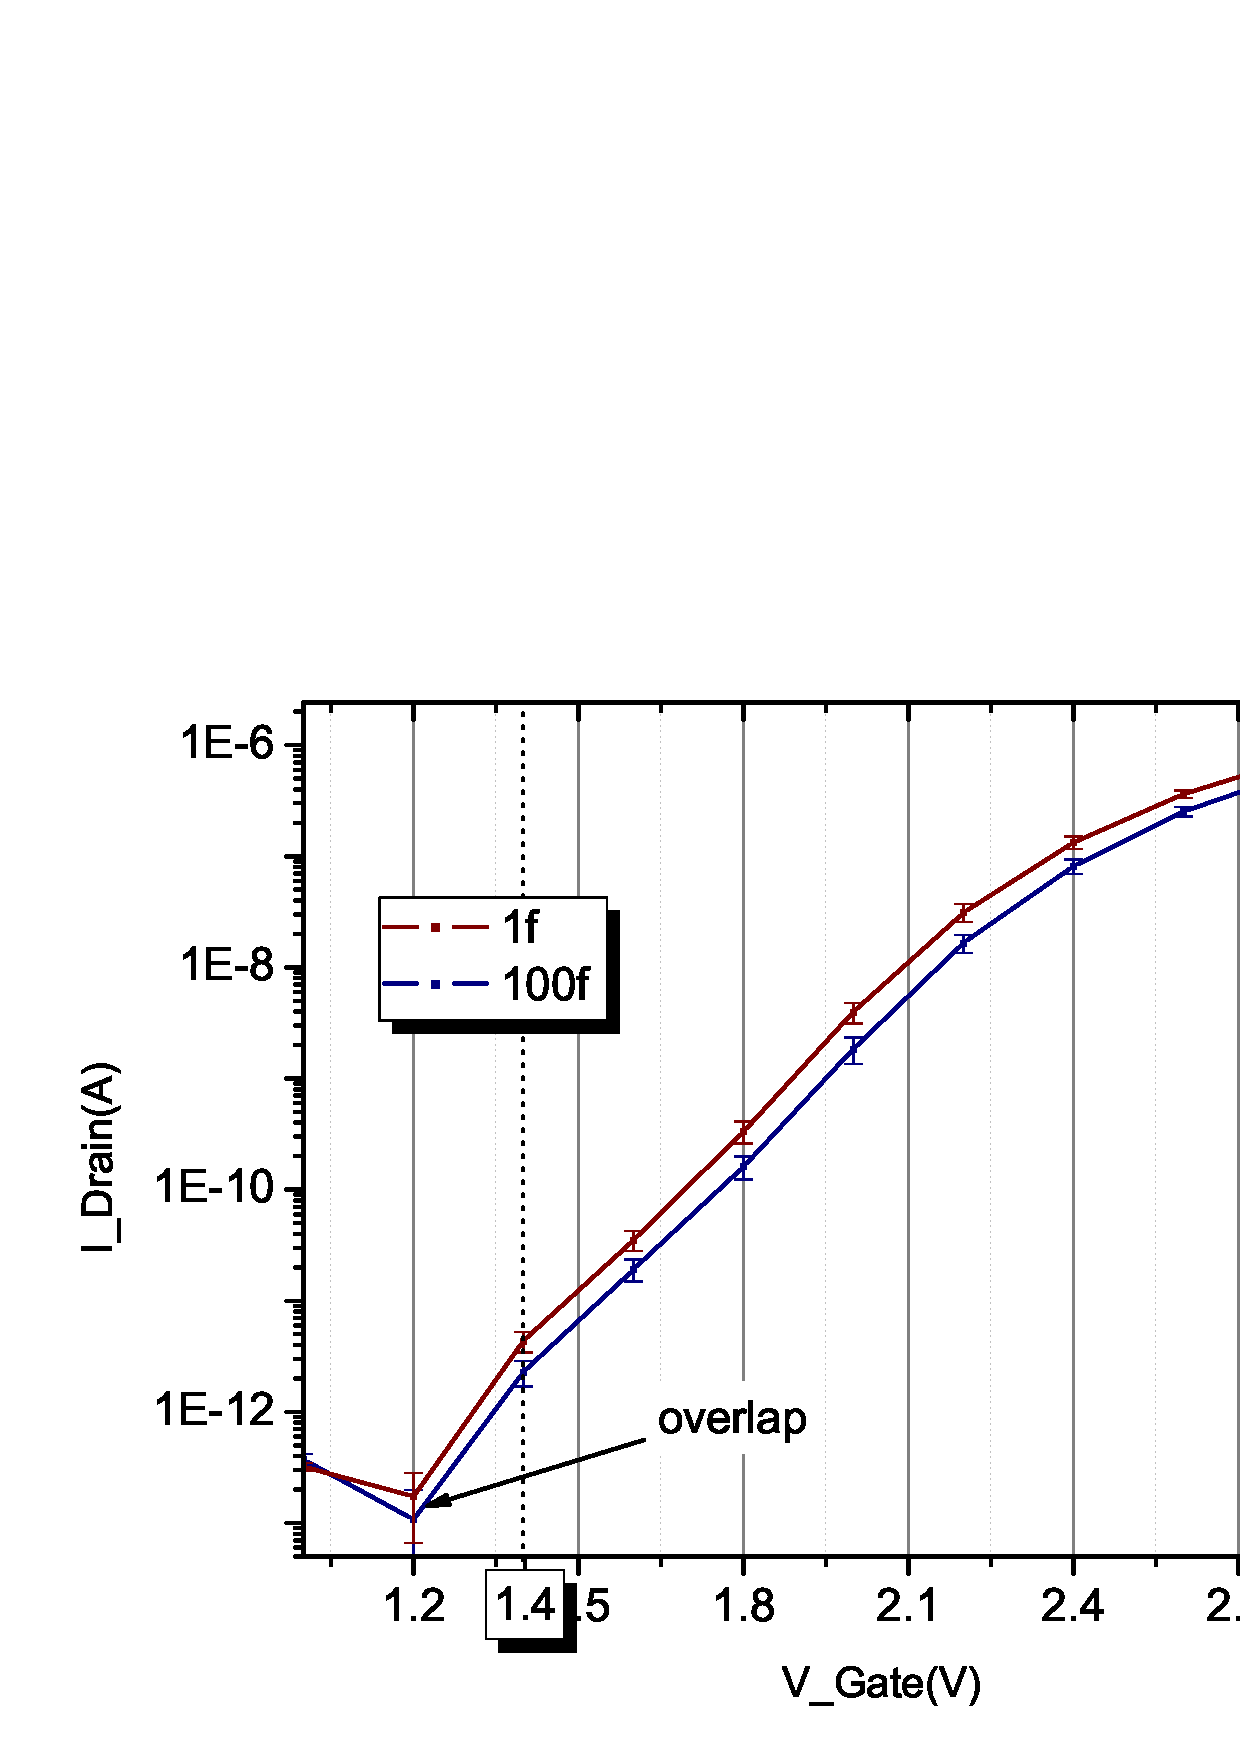
\includegraphics[scale=0.3]{images/chapter3/208_devices/L2-8_log.png}
        (a)
    \end{minipage}
    \hfill
    \begin{minipage}[t]{0.4\textwidth}
        \centering
        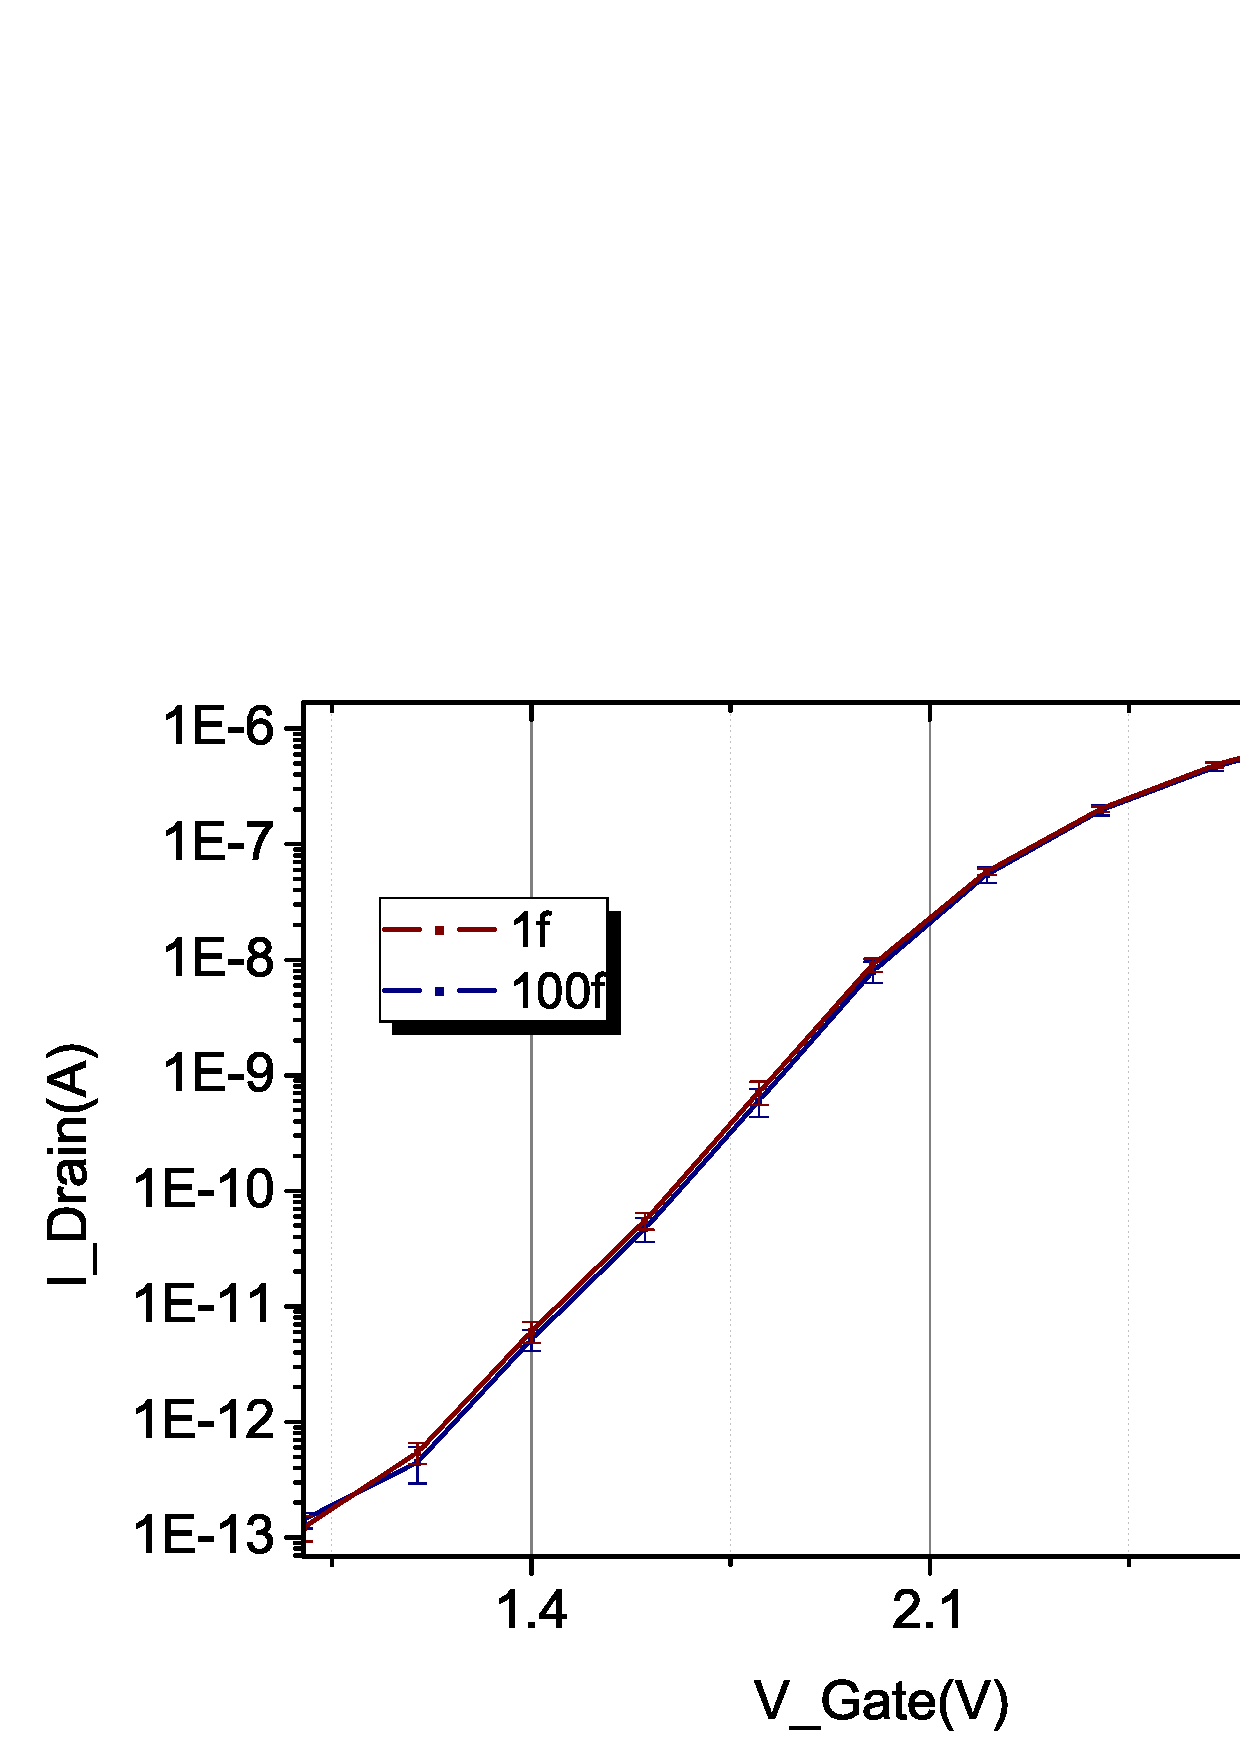
\includegraphics[scale=0.3]{images/chapter3/208_devices/L2-10_log.png}
        (b)
    \end{minipage}
    \caption{}
    \label{fig:SD_sucandfail}
\end{figure}

The Fig.\ref{fig:SD_sucandfail} are concentration-dependent measurements (1 femto mole(fM) and 100fM biomolecule solution) obtained with two elements ((a) and (b)).
The two curves in the (a) are distinguishable from the other after gate voltage of 1.4v
They are not distinguishable in the (b) since they overlap each other.
We thus assert that the element of (b) can't detect the concentration difference between 1fM and 100fM.
The noise is stronger than the signal (The signal means the $I_D$ difference caused by the concentration difference).
The element of (a) is able to do so if it is biased at gate voltage larger than 1.4v or drain current larger than 1E-11.

\begin{figure}[!htbp]
        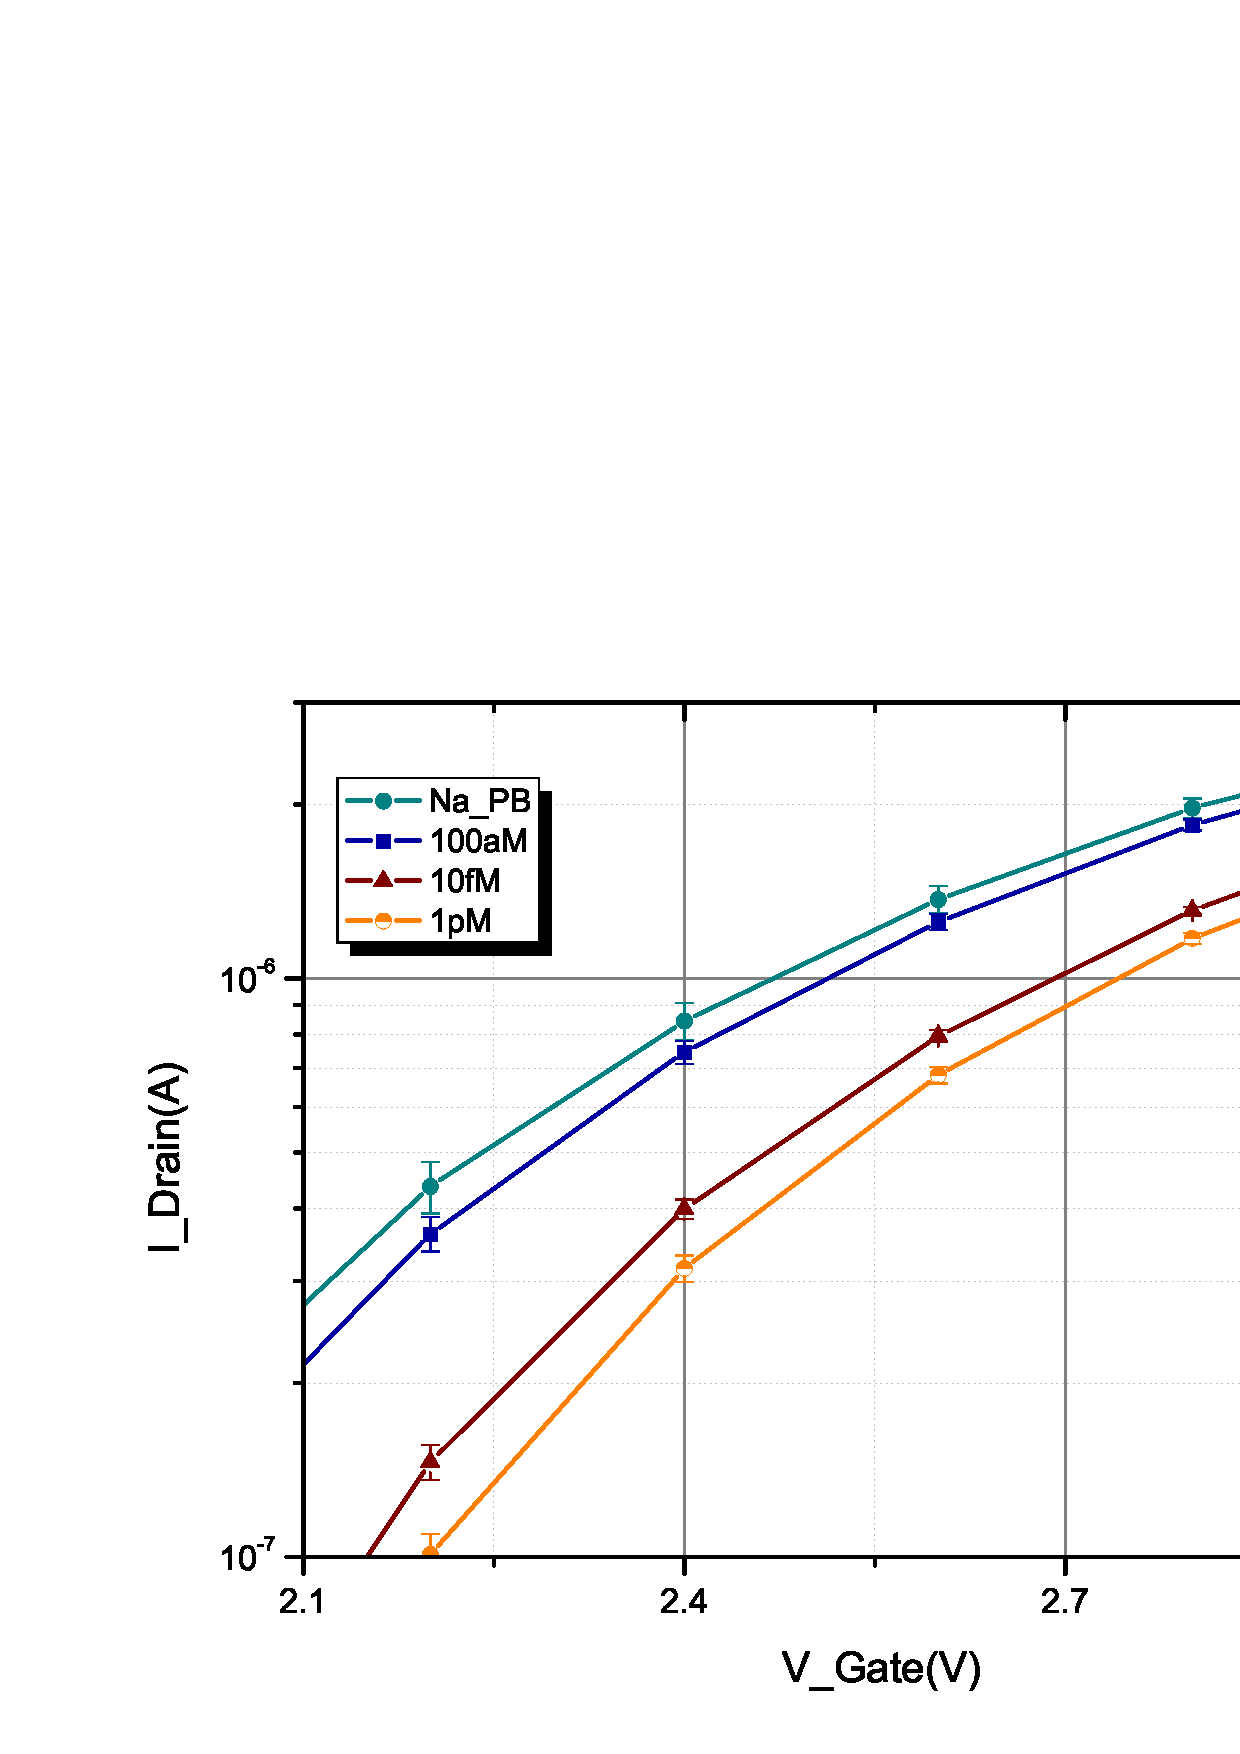
\includegraphics[width=1\textwidth]{images/chapter3/128_allT_mag.png}
    \caption{}
    \label{fig:SD_allT}
\end{figure}

In Fig.\ref{fig:SD_allT}, the $I_D$ increase with the biomolecule concentration.
One can find that there are only few ``space'' between PBS buffer and solution containing biomolecule with concentration of 100aM.
Hence the 100aM should be the limit of detection.

It is worth noting that there are more space between 100aM and 10fM than the space between 10fM and 1 pico mole(pM).
We calculate the noise rate: ${SD} / {Mean}$ which seems independent of concentration (Fig.\ref{fig:SD_allT2}).
{\color{red}These implies that the ``resolution'' for detecting concentration ranging from 100aM to 10fM may be better than the that ranging from 10fM to 1pM.}
\begin{figure}[!htbp]
        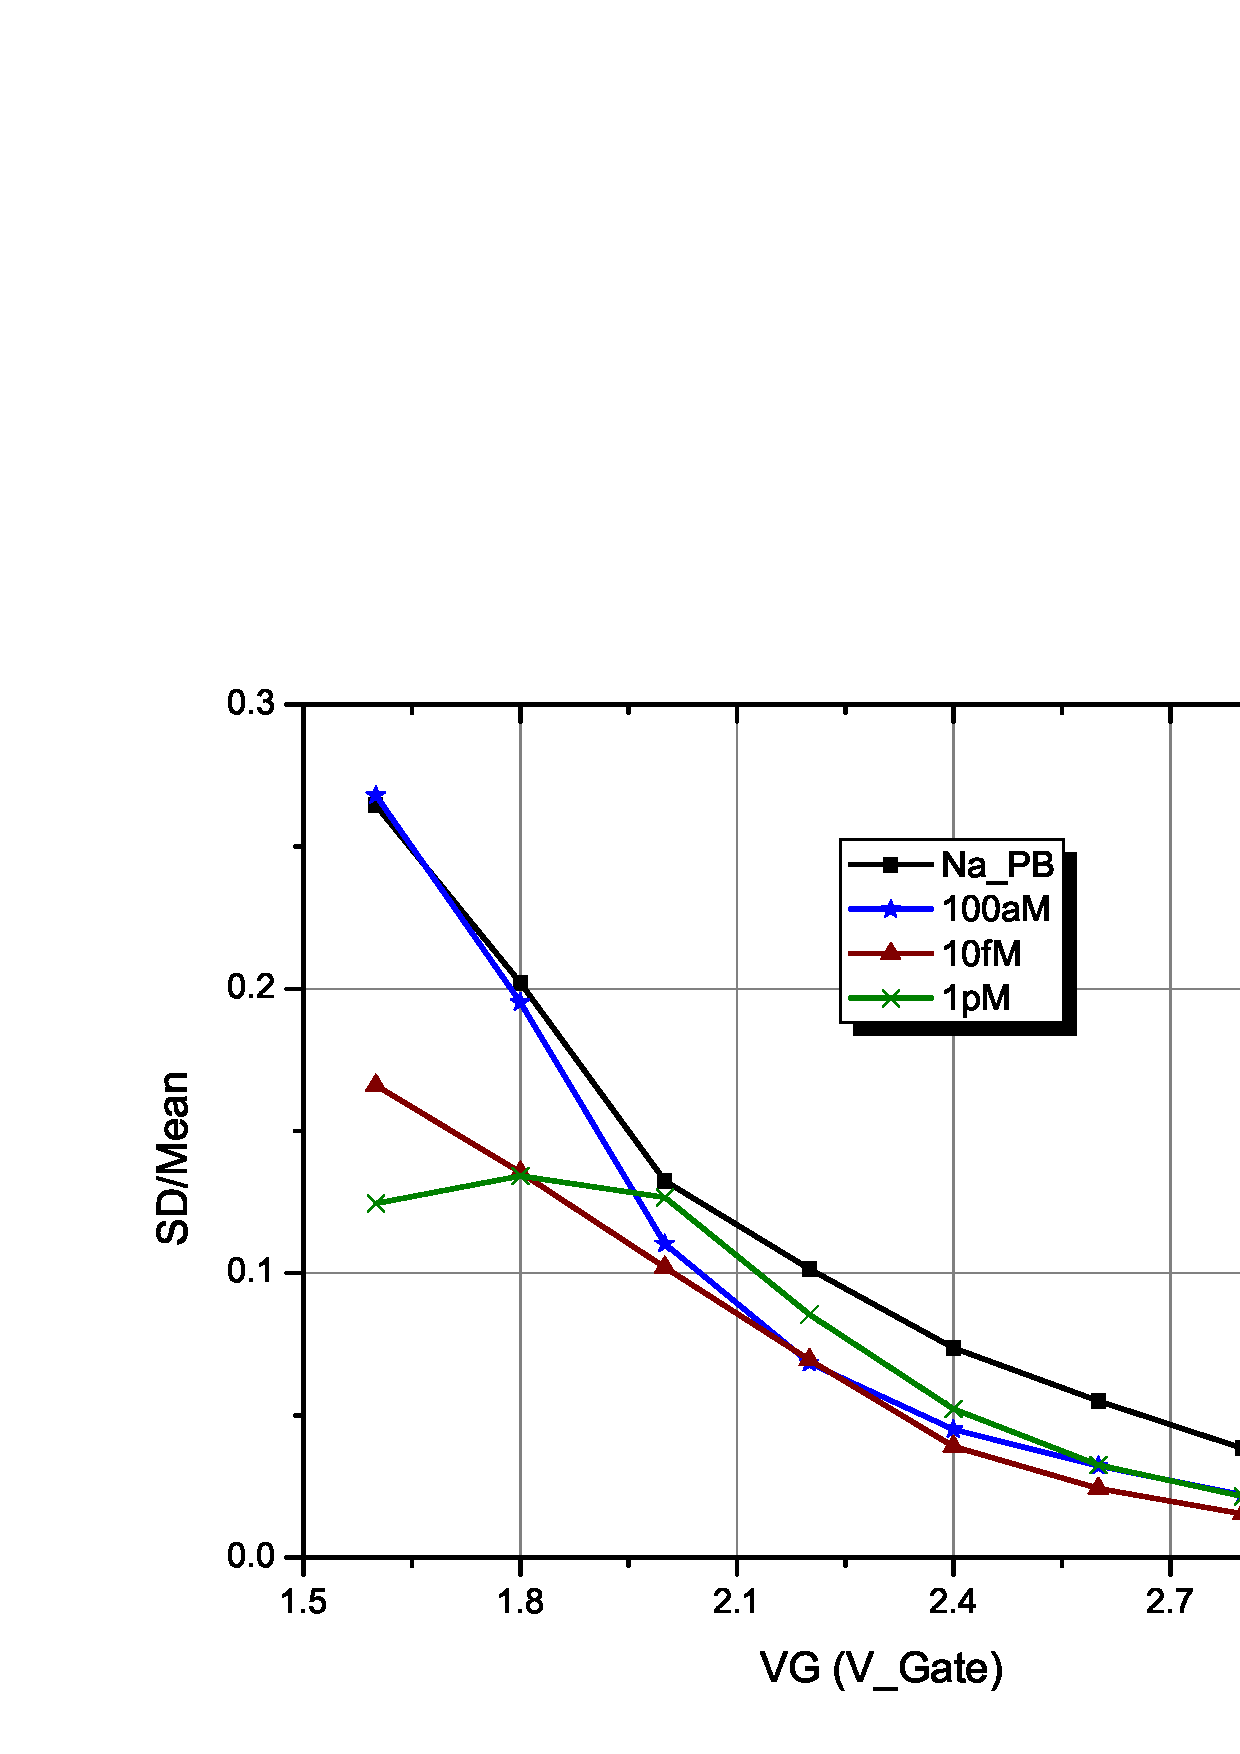
\includegraphics[width=1\textwidth]{images/chapter3/128_allT_error.png}
    \caption{}
    \label{fig:SD_allT2}
\end{figure}





\subsection*{Appropriate Bias Gate Voltage}
In \cite{C6}, the team found that ``the induced change of current ($I_D$) following biomolecule was dependent on the applied gate voltage (VG)''.
The team tried to find a bias gate voltage range which can induce more current response.
By taking noise into consideration, we proposed that one should choose the region with more ``noise tolerance''.
We define the noise tolerance as below:
\setlength{\mathindent}{2cm}
\begin{align}
    noise \quad tolerance = \frac{I_D1 - SD1 - (I_D2 + SD2)}{I_D2}
\end{align}
$I_D$ and $SD$ are the mean and standard deviation of a curve.
The larger the noise tolerance implies there are more space between two curves.

The Fig.\ref{fig:SD_Device}(c), (f), (i) are the noise tolerance of Fig.\ref{fig:SD_Device}(a), (d), (g).
The Fig.\ref{fig:SD_Device}(b), (e), (h) are the noise rate respectively.
We observe a rising trend in both noise rate and noise tolerance as gate voltage decrease.
Moreover, a small peak appears in (c) and (f) located around the section where transistor switches from weak inversion region to strong inversion region.
We therefore suggest that this section should be the best region under which nanowire should be operated.


\begin{figure}[!hbtp]
    \centering
    \begin{minipage}[t][20cm][t]{1\textwidth}
        \begin{minipage}[t]{0.3\textwidth}
            \centering
            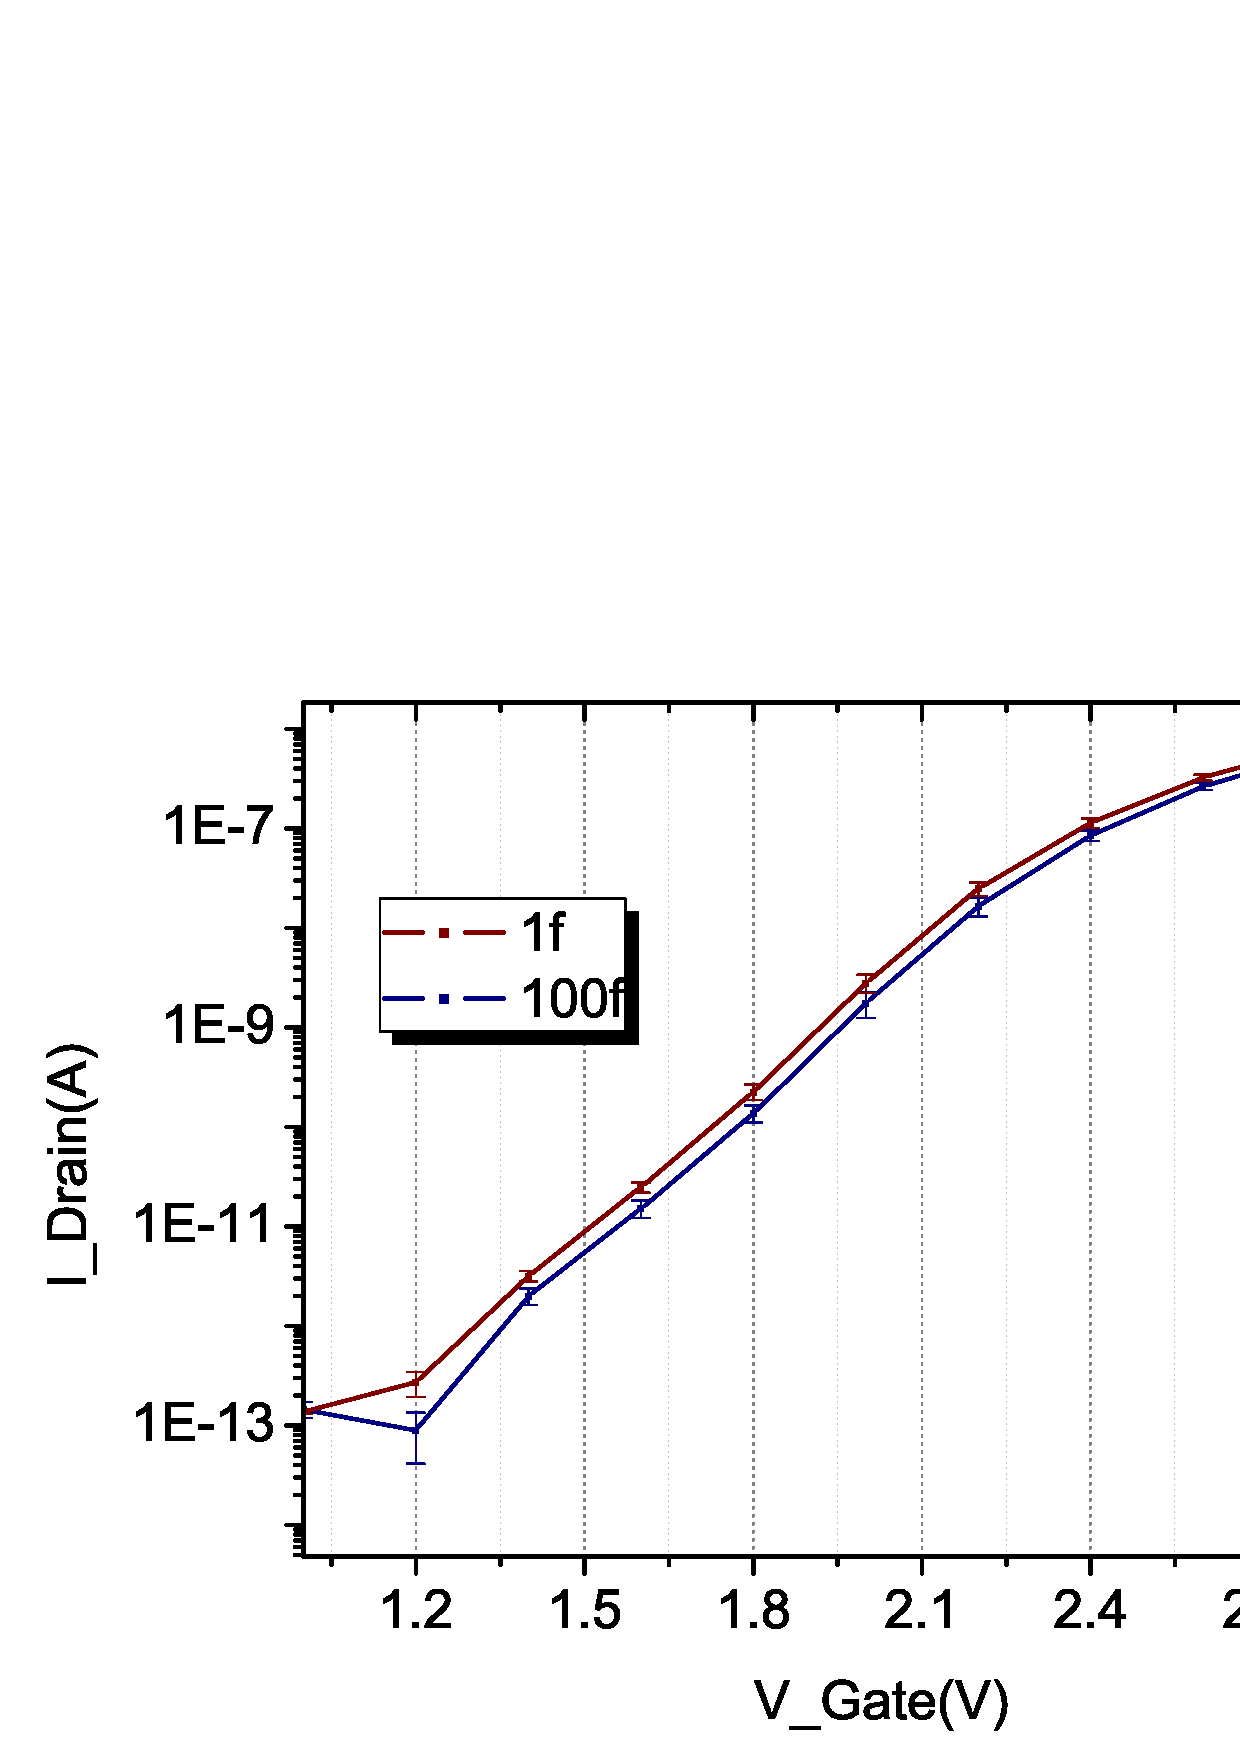
\includegraphics[width=1.5\textwidth]{images/chapter3/208_devices/L2-7_log.png}
            (a)
        \end{minipage}
        \hfill
        \begin{minipage}[t]{0.3\textwidth}
            \centering
            \includegraphics[width=1.5\textwidth]{images/chapter3/208_devices/L2-7_error.png}
            (b)
        \end{minipage}
        \hfill
        \begin{minipage}[t]{0.3\textwidth}
            \centering
            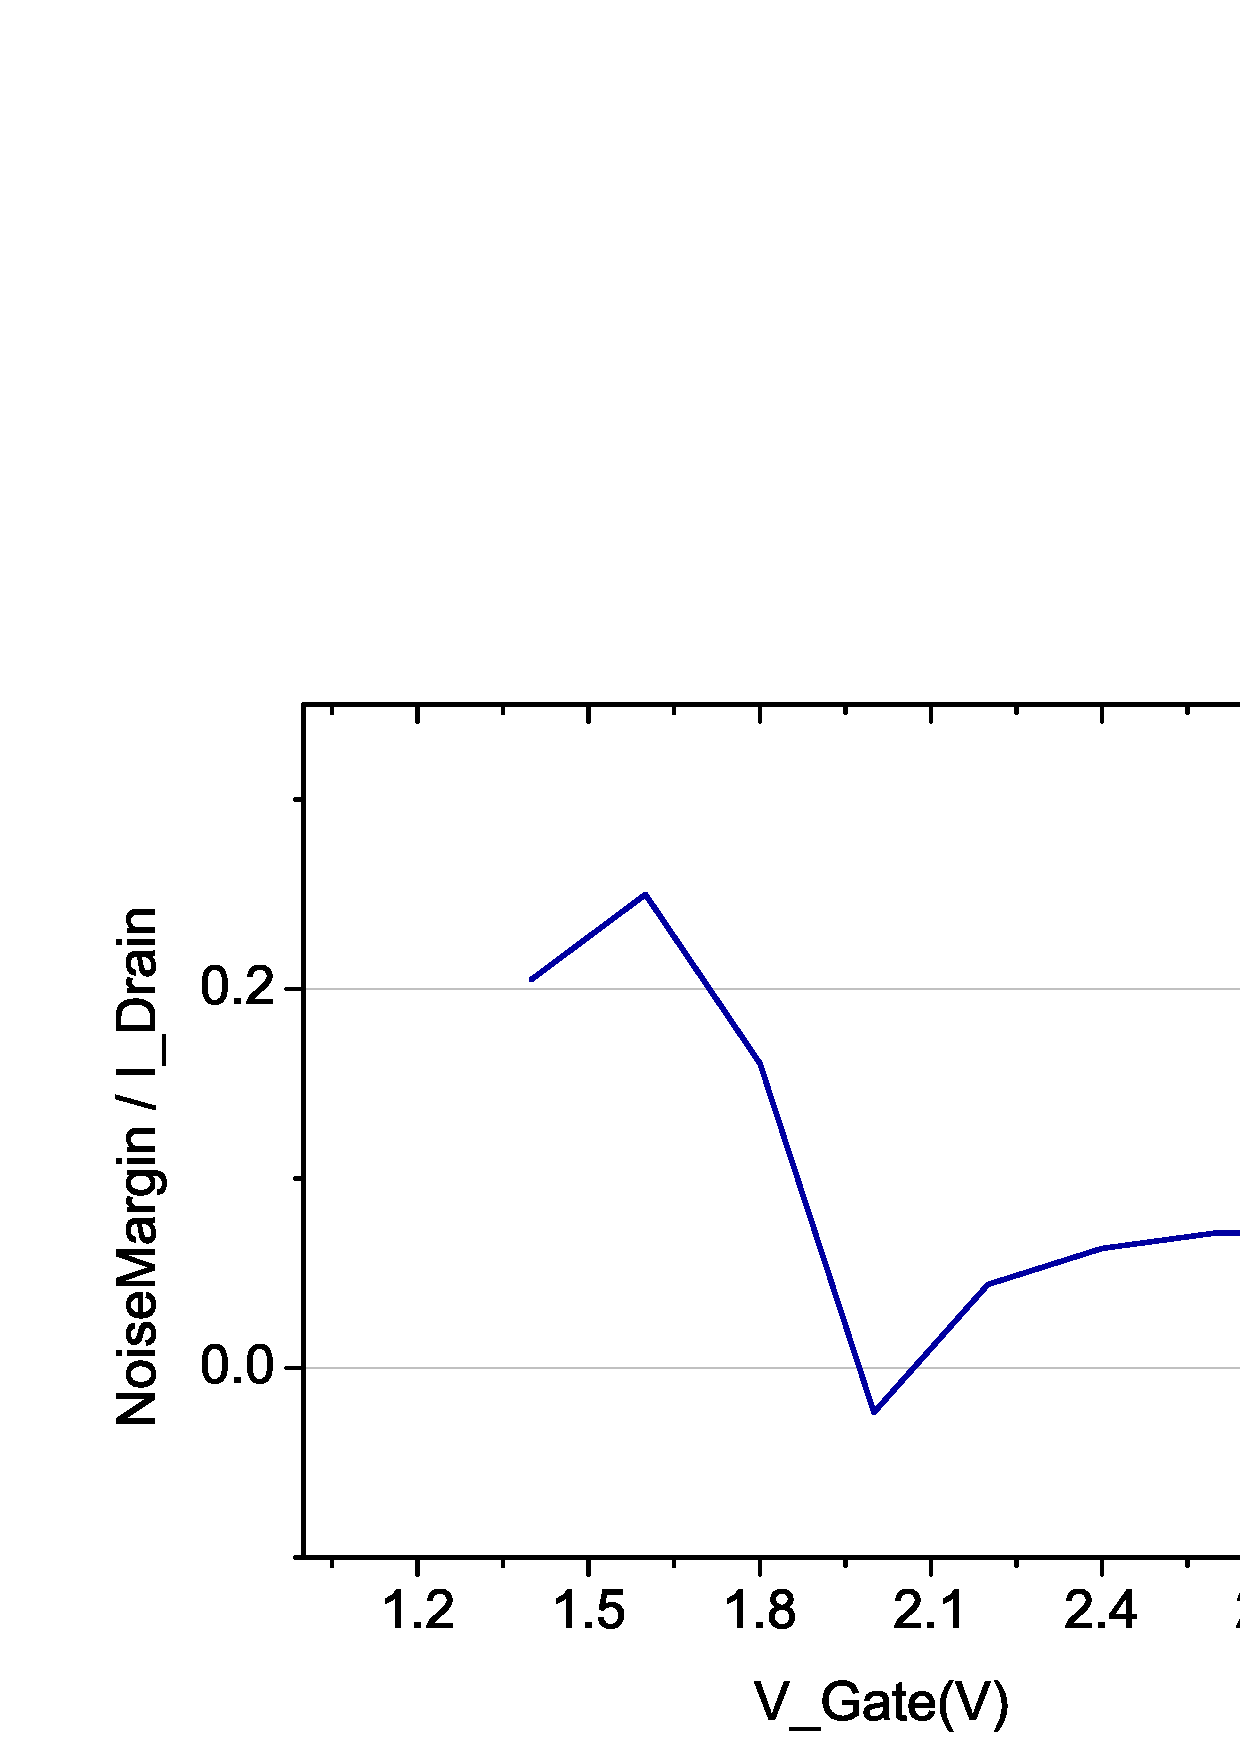
\includegraphics[width=1.5\textwidth]{images/chapter3/208_devices/L2-7_margin.png}
            (c)
        \end{minipage}
        \vfill
        \begin{minipage}[t]{0.3\textwidth}
            \centering
            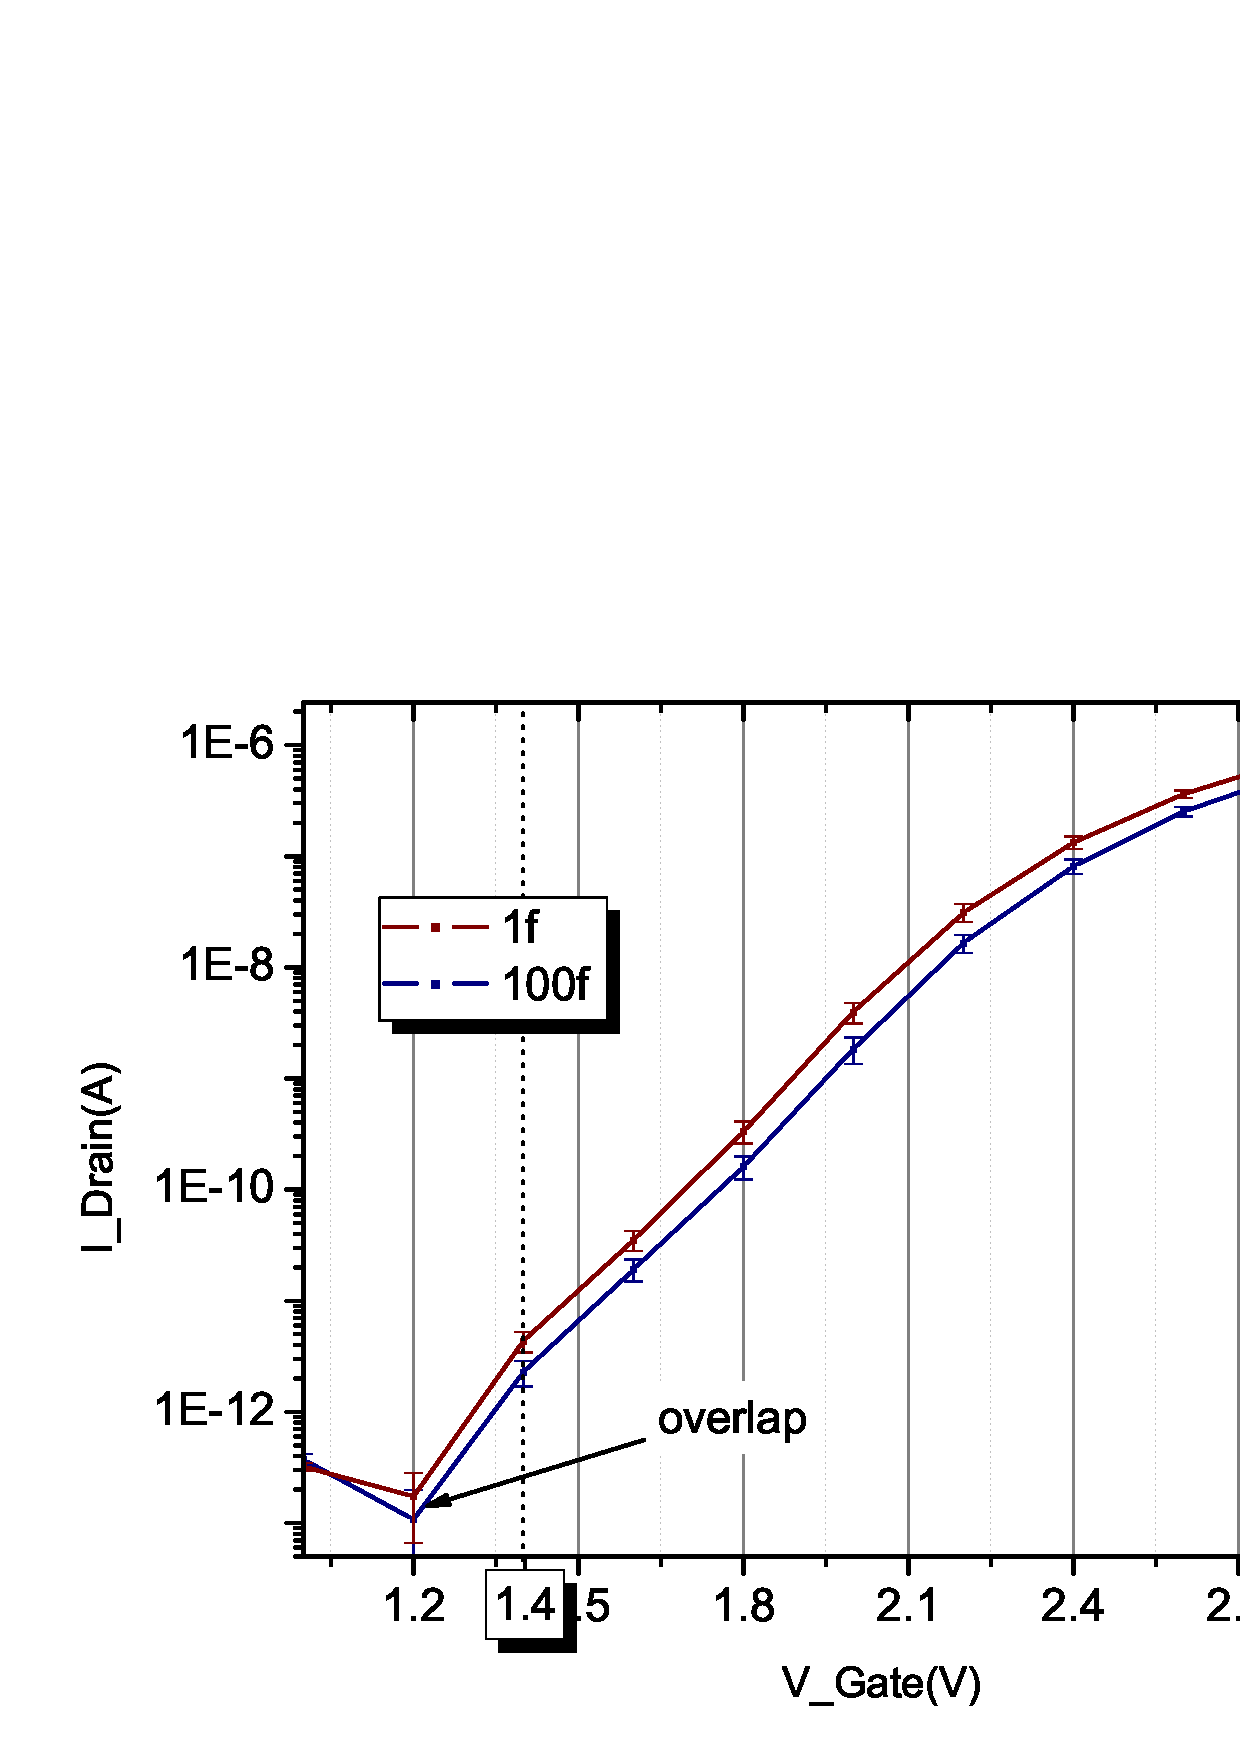
\includegraphics[width=1.5\textwidth]{images/chapter3/208_devices/L2-8_log.png}
            (d)
        \end{minipage}
        \hfill
        \begin{minipage}[t]{0.3\textwidth}
            \centering
            \includegraphics[width=1.5\textwidth]{images/chapter3/208_devices/L2-8_error.png}
            (e)
        \end{minipage}
        \hfill
        \begin{minipage}[t]{0.3\textwidth}
            \centering
            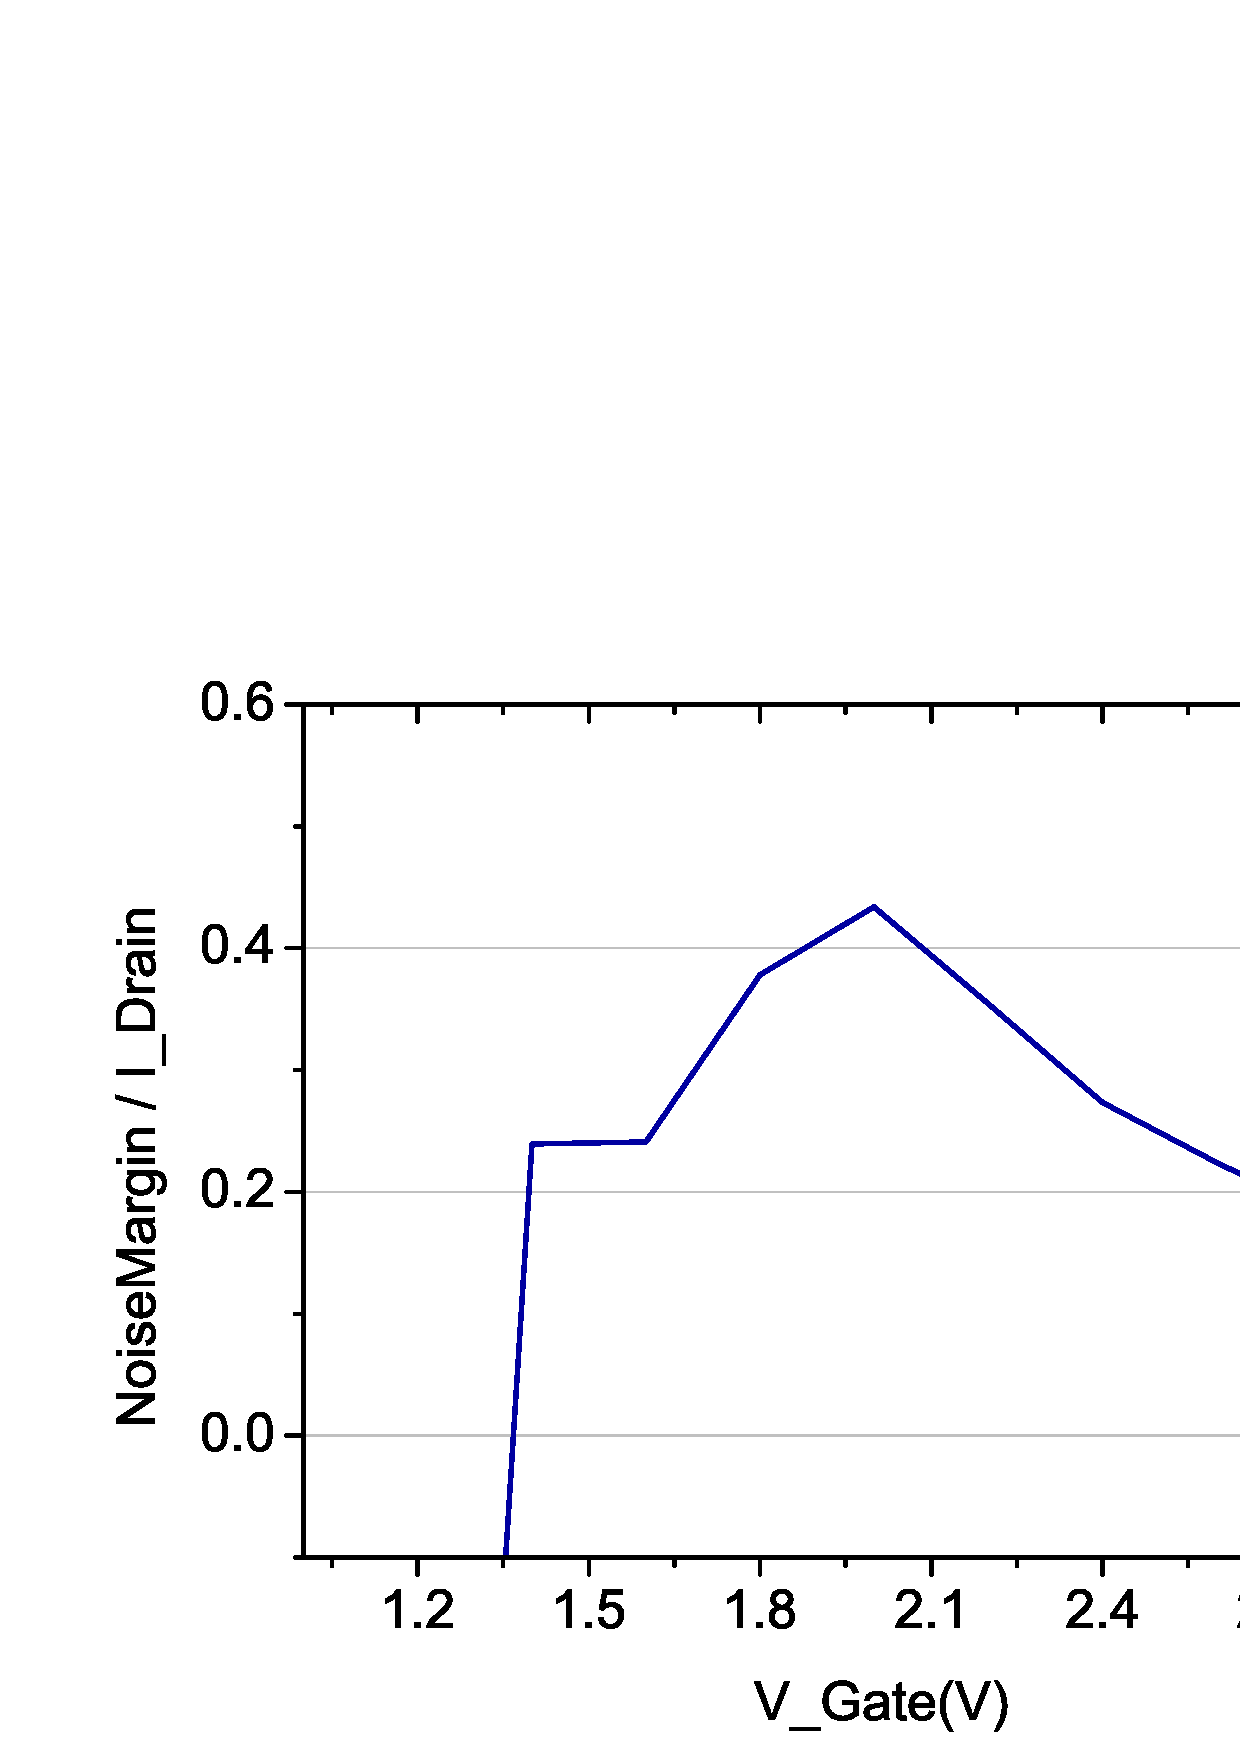
\includegraphics[width=1.5\textwidth]{images/chapter3/208_devices/L2-8_margin.png}
            (f)
        \end{minipage}
        \vfill
        \begin{minipage}[t]{0.3\textwidth}
            \centering
            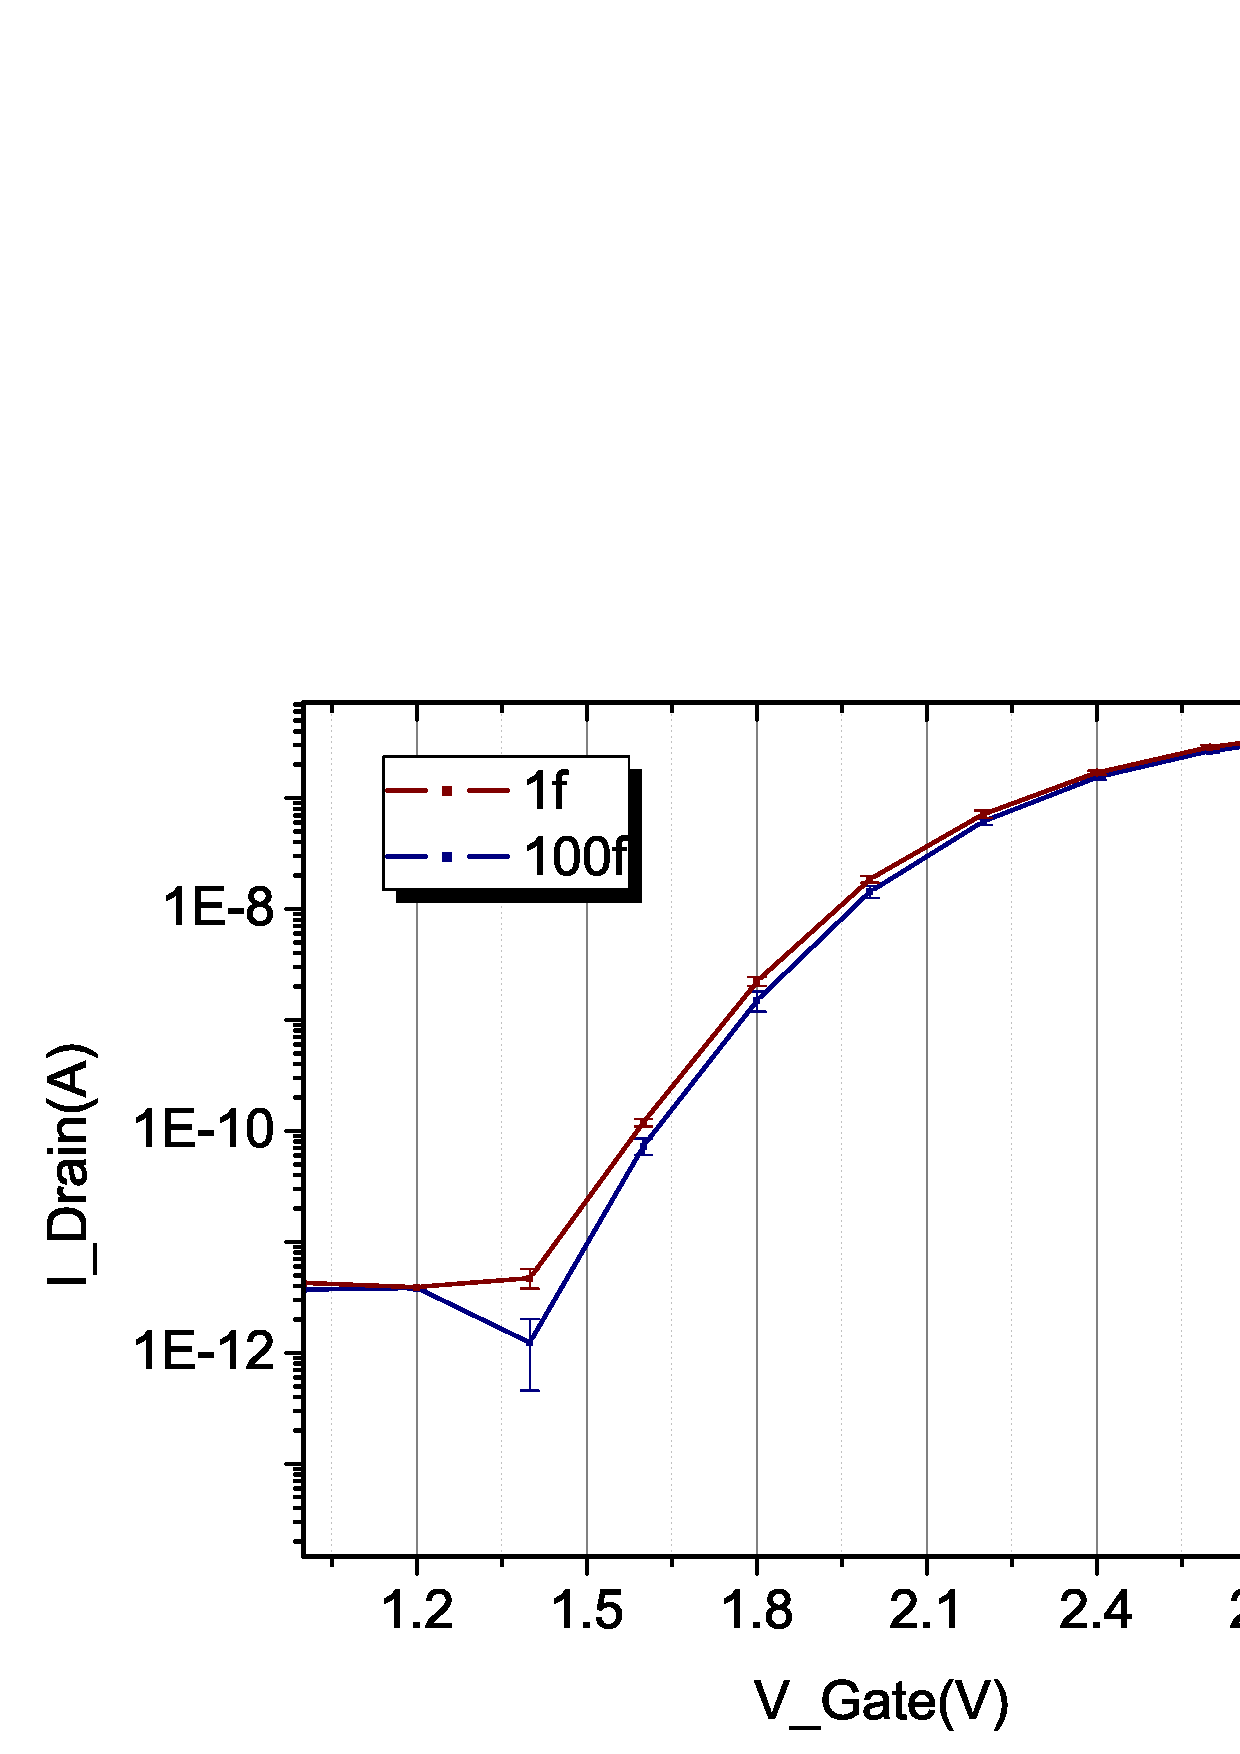
\includegraphics[width=1.5\textwidth]{images/chapter3/208_devices/L2-12_log.png}
            (g)
        \end{minipage}
        \hfill
        \begin{minipage}[t]{0.3\textwidth}
            \centering
            \includegraphics[width=1.5\textwidth]{images/chapter3/208_devices/L2-12_error.png}
            (h)
        \end{minipage}
        \hfill
        \begin{minipage}[t]{0.3\textwidth}
            \centering
            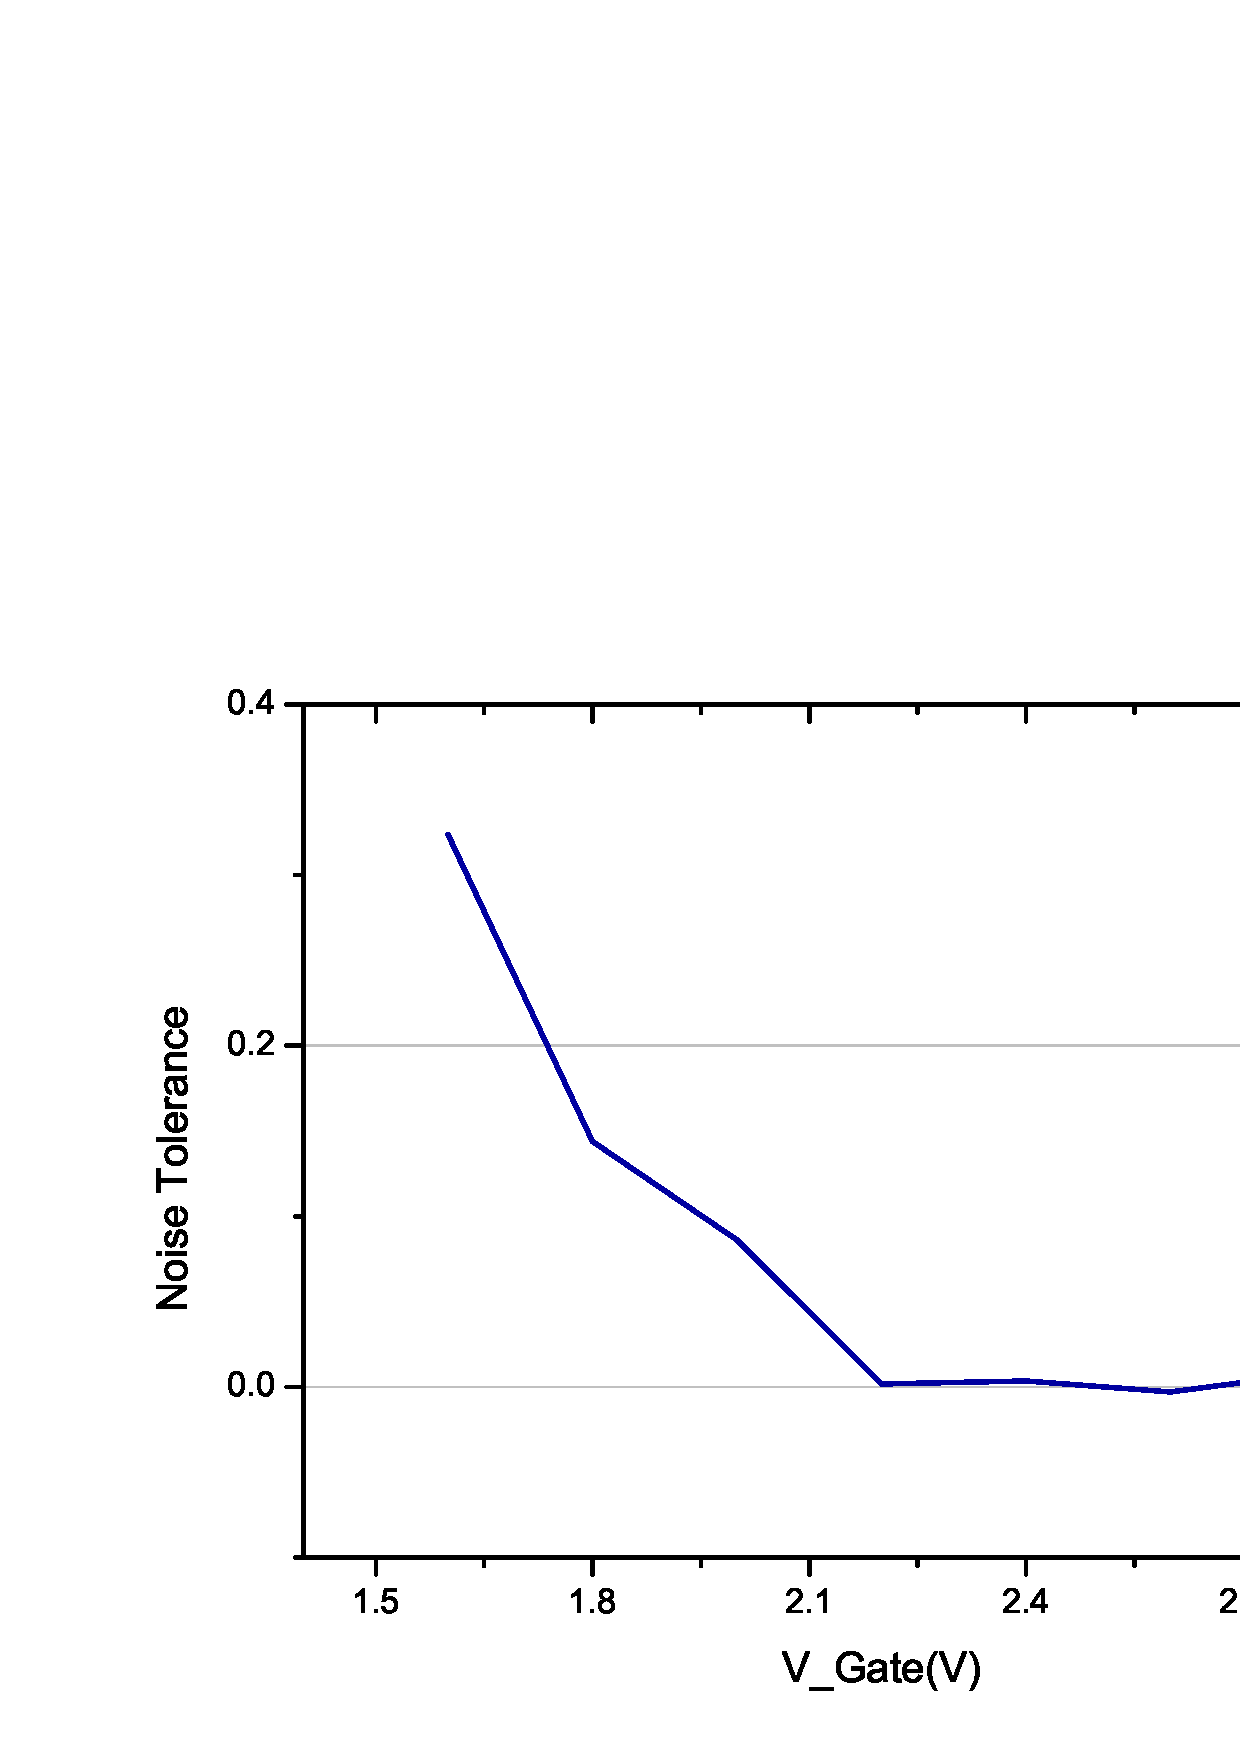
\includegraphics[width=1.5\textwidth]{images/chapter3/208_devices/L2-12_margin.png}
            (i)
        \end{minipage}

    \end{minipage}
    \caption{}
    \label{fig:SD_Device}
\end{figure}



\section{Electrical Measurements}
This section presents the results.

\subsection*{Front Gate and Back Gate}
Two gates are available: floating gate (liquid gate) and back-gate.
We choose floating gate as the operation gate in spite of some advantages that back-gate has.
One of them is the ability to lower the 1/f noise \cite{C7, C8}.
However, this only happens in a very high gate voltage, which is not practical in the integrated circuit design.
Moreover, the floating gate induces larger drain-current.
In other words, it has higher transconductance. And a high transconductance leads to a stronger feedback ability in our design.

% \begin{figure}[!htbp]
%     \centering
%     {\fontfamily{pag}\selectfont\textbf{
%         \def\svgwidth{5.0cm}
%         \fontsize{6}{7}\selectfont
%         \input {images/FgBg_Compare_Id_dev.pdf_tex}
%     }}
%     \fontsize{6}{7}\selectfont
%     \caption{}
%     \label{fig:res}
% \end{figure}
%
% \begin{figure}[!htbp]
%     \centering
%     {\fontfamily{pag}\selectfont\textbf{
%         \def\svgwidth{5.0cm}
%         \fontsize{6}{7}\selectfont
%         \input {images/FgBg_Compare_Id.pdf_tex}
%     }}
%     \fontsize{6}{7}\selectfont
%     \caption{}
%     \label{fig:res}
% \end{figure}


\begin{figure}[!htbp]
    \centering
    \begin{minipage}[t][0.1\textheight]{1\textwidth}
        \centering
        \def\svgwidth{10cm}
        \fontsize{6}{15}\selectfont
        \input {images/FgBg_Compare_Id.pdf_tex}
        (a)
    \end{minipage}
    \vfill
    \begin{minipage}[t][0.1\textheight]{1\textwidth}
        \centering
        \def\svgwidth{10cm}
        \fontsize{6}{15}\selectfont
        \input {images/FgBg_Compare_Id_dev.pdf_tex}
        (b)
    \end{minipage}
    \caption{}
    \label{fig:IdVgandgbsId}
\end{figure}

\subsection{Parameters}
The most crucial parameter for our circuit design is the transconductance (gm).
{\color{red}
    The gm is acquired by finding the relation between drain-to-source current ($I_d$) and gate-source voltage ($V_g$), and perform differentiation: $\frac{\partial I_d}{\partial V_g}$.
    use standard PBS as
}

\begin{figure}[!htbp]
    \centering
    \begin{minipage}[t][0.1\textheight]{1\textwidth}
        \centering
        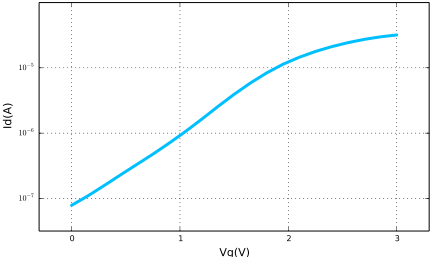
\includegraphics[width=0.6\textwidth,natwidth=610,natheight=442]{images/pIdVg.png}
        (a)
    \end{minipage}
    \hfill
    \begin{minipage}[t][0.1\textheight]{1\textwidth}
        \centering
        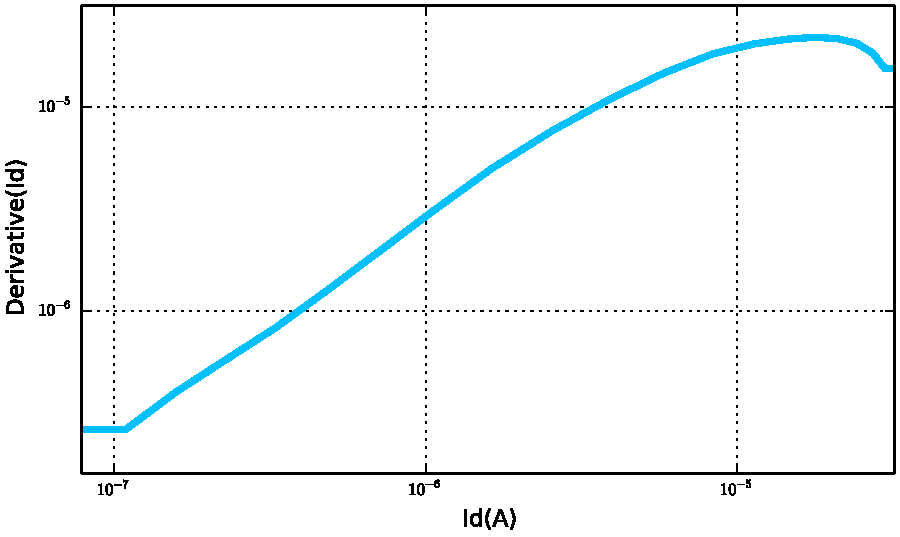
\includegraphics[width=0.6\textwidth,natwidth=610,natheight=442]{images/pIdgbs.png}
        (b)
    \end{minipage}
    \caption{}
    \label{fig:pIdVg}
\end{figure}

The Id-Derivative figures indicates there is a ``linear region'' where gm is proportional to Id.
This property implies the transconductance can be controlled in simple way.
As mentioned in introduction, we may find specific bias Id for distinct elements and adjust their transconductance to a same value.



We also prove that the transconductance under this region is unaffected by the drain-source voltage variance.

\begin{figure}[!htbp]
    \centering
    % {\fontfamily{pag}\selectfont\textbf{
        % \def\svgwidth{10cm}
        % \fontsize{6}{10}\selectfont
        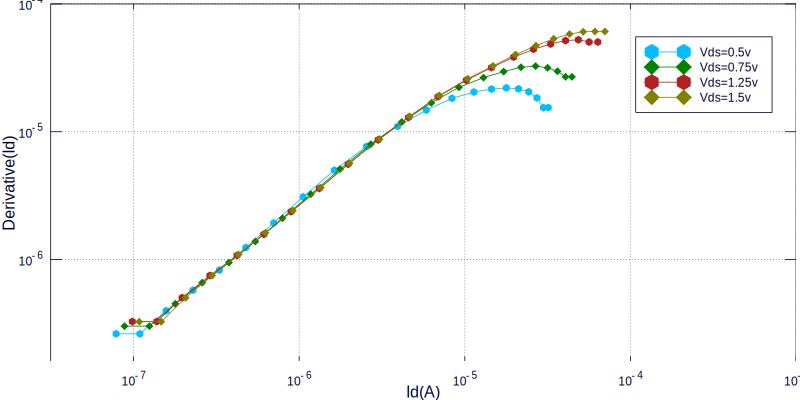
\includegraphics[width=0.8\textwidth,natwidth=610,natheight=642]{images/pIdgbs_Vd.png}
    % }}
    \fontsize{6}{10}\selectfont
    \caption{Id-transconductance with Vds variance}
    \label{fig:Idgbs_Vd}
\end{figure}




\begin{figure}[!htbp]
    \centering
    % {\fontfamily{pag}\selectfont\textbf{
    \def\svgwidth{10cm}
    \fontsize{6}{10}\selectfont
    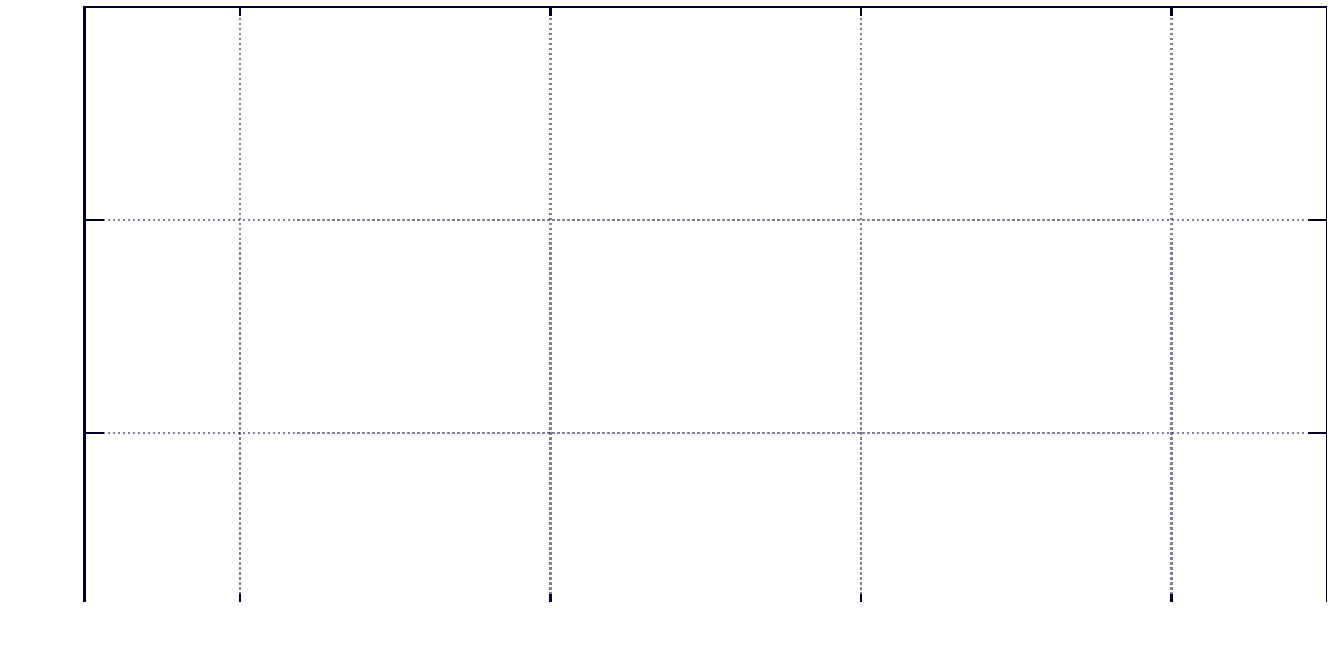
\includegraphics[width=0.8\textwidth,natwidth=610,natheight=642] {images/pDisparity.png}
    % }}
    \fontsize{6}{10}\selectfont
    \caption{Distinct element with a line idicate they have same transconductance}
    \label{fig:disparity}
\end{figure}
By measuring two nanowire element which lie on the same wafer and are immersed with the same testing PBS solution









 

